% \documentclass[11pt,a4paper,uplatex,twoside,dvipdfmx]{ujarticle} 	% for uplatex
% \documentclass[11pt,a4paper,twoside,dvipdfmx]{jarticle}		% platex
\documentclass[11pt,a4paper,twoside,dvipdfmx]{jsarticle}   % 美文書
%==== 科研費LaTeX =============================================
%	2020(H32)年度 PD
%============================================================
% 2008-03-08: Taku Yamanaka (JSPS Research Center for Science Systems / Osaka Univ.)
% 2008-03-10: Taku; Fixed a bug which was missing p.7.
% 2009-03-04: K.S.: Revised for JFY2010.
% 2010-03-04: Taku: Revised for JFY2011.
% 2011-03-20: Taku: Revised for JFY2012.
% 2012-02-25: Taku: Revised for JFY2013.
% 2013-03-14: Taku: Revised for JFY2014.
% 2014-03-02: Taku: Revised for JFY2015.
% 2015-02-23: Taku: Revised for JFY2016.
% 2016-02-26: Taku: Revised for JFY2017.
%============================================================
%=======================================
% form00_header.tex
%	General header for kakenhiLaTeX,  Moved over from form00_2010_header.tex.
%	2009-09-06 Taku Yamanaka (Osaka Univ.)
%==== General Version History ======================================
% 2006-05-30 Taku Yamanaka (Physics Dept., Osaka Univ.)
% 2006-06-02 V1.0
% 2006-06-14 V1.1 Use automatic calculation for cost tables.
% 2006-06-18 V1.2 Split user's contents and the format.
% 2006-06-20 V1.3 Reorganized user and format files
% 2006-06-25 V1.4 Readjusted all the table column widths with p{...}.
%				With \KLTabR and \KLTabRNum, now the items can be right-justified
%				in the cell defined by p{...}.
% 2006-06-26 V1.5 Use \newlength and \setlength, instead of \newcommand, to define positions.
% 2006-08-19 V1.6 Remade it for 2007 JFY version.
% 2006-09-05 V1.7 Added font declarations suggested by Hoshino@Meisei Univ.
% 2006-09-06 V1.8 Introduced usePDFform flag to switch the form file format.
% 2006-09-09 V1.9 Changed p.7, to allow different heights between years. (Thanks to Ytow.)
% 2006-09-11 V2.0 Added an option to show budget summary.
% 2006-09-13 V2.1 Added an option to show the group.
% 2006-09-14 V2.1.1 Cleaned up Kenkyush Chosho.
% 2006-09-21 V2.2 Generated under a new automatic development system.

% 2007-03-24 V3.0 Switched to a method using "picture" environment.

% 2007-08-14 V3.1 Switched to kakenhi3.sty.
% 2007-09-17 V3.2 Added \KLMaxYearCount
% 2008-03-08 V3.3 Remade it for 2009 JFY version\
% 2008-09-08 V3.4 Added \KLXf ... \KLXh.
% 2011-10-20 V5.0 Use kakenhi5.sty, to utilize array package in tabular environment.
% 2012-08-14 v5.1 Moved preamble and kakenhi5 into the current directory, instead of the parent directory.
% 2012-11-10 v6.0 Switched to kakenhi6.sty.
% 2015-08-26 v6.1 Added KLFirstPageIsLongPage flag.
% 2018-02-12 Taku: Commented out \DeclareFontShape ...
%=======================================
%============================================================
% preamble.tex
%
% Dummy section and subsection commands.
% With these, some editors (such as TeXShop, etc.) can jump to the (sub)sections.
\newcommand{\dummy}{dummy}% 
\renewcommand{\section}[1]{\renewcommand{\dummy}{#1}}
\renewcommand{\subsection}[1]{\renewcommand{\dummy}{#1}}

% Flag for switching form file format.......
\usepackage{ifthen}
\newboolean{usePDFform}
\newboolean{BudgetSummary}

\usepackage{forms/kakenhi6}

\pagestyle{empty}

% ===== Parameters for LaTeX =========================

% ===== Font declarations  ======================================
%%\DeclareFontShape{JT1}{mc}{m}{it}{<->ssub * mc/m/n}{}
%%\DeclareFontShape{JY1}{mc}{m}{it}{<->ssub * mc/m/n}{}

% ===== Parameters for KL (Kakenhi LaTeX) ========================
% general purpose temporary variables	-2007
\newcommand{\KLX}{}
\newcommand{\KLXa}{}
\newcommand{\KLXb}{}
\newcommand{\KLXc}{}
\newcommand{\KLXd}{}
\newcommand{\KLXe}{}
\newcommand{\KLXf}{}
\newcommand{\KLXg}{}
\newcommand{\KLXh}{}
\newcommand{\KLY}{}
\newcommand{\KLYa}{}
\newcommand{\KLYb}{}
\newcommand{\KLYc}{}
\newcommand{\KLYd}{}
\newcommand{\KLYe}{}
\newcommand{\KLYf}{}
\newcommand{\KLXR}{}
\newlength{\KLCella}
\newlength{\KLCellb}
\newlength{\KLCellc}
\newlength{\KLCelld}
\newlength{\KLCelle}
\newlength{\KLCellf}
\newlength{\KLCellg}
\newlength{\KLCellh}

% sub-page
\newlength{\KLSubPageX}
\newlength{\KLSubPageY}
\newlength{\KLspx}
\newlength{\KLspy}
\newcommand{\KLSubPageXmm}{}	% for \input(x,y){....} which uses a unit (mm)
\newcommand{\KLSubPageYmm}{}	% for \input(x,y){....} which uses a unit (mm)

% margins for parbox inside frames; in units of points
\newcounter{KLParboxSideMargin}
\newcounter{KLParboxTopMargin}
\newcounter{KLParboxBottomMargin}

% ===== standard counters ======================================
\newcounter{KLSubPageNo}	% sub-page counter
\newcounter{KLPageOffset}		% to generate sub-page number
\newcounter{KLMaxYearCount}	% # of years for the proposal

% ===== standard flags ============================
\newboolean{KLFirstPageIsLongPage}

% ===== initializations ============
\KLInitTypesettingPageSelection
\newcommand{\KLCLLang}{}	% language-dependent left-justification in tabular



% user01_header
%=== 様式のファイルの形式の指定 =================
%   PDFではなく、eps の様式を読み込む場合は、次の行の頭に「%」をつけてください。
\setboolean{usePDFform}{true}
%===================================
%==========================================================
% form01_header.tex
%	2014-03-02: Taku Yamanaka (Osaka Univ.)
%		This is called after usePDFform is set.
%		Originally, this part was in form07_header.tex, but then
%		\usepackage{color} that is called before it was not effective.
%		[dvipdfmx] is not used for eps forms, because it makes the forms
%		slightly larger than pdf forms.
%		
%==========================================================
% ===== File format for forms ===========================
\ifthenelse{\boolean{usePDFform}}{
	\newcommand{\KLFormFormat}{pdf}	\usepackage[dvipdfmx]{graphicx}
}{	\newcommand{\KLFormFormat}{eps}	\usepackage{graphicx}
}

%----------------------------------------------------------------------------


% user02_header
%=== 予算の表の印刷 =====================
% 予算の集計の表を出すためには、次の行の頭の%を消してください。
%\setboolean{BudgetSummary}{true}
%=================================

%=== For English, uncomment the next line to left-justify inside table columns.
%\renewcommand{\KLCLLang}{\KLCL}

% === 一部のページだけタイプセット ==============
% New in 2009 fall version!
% 選んだページだけタイプセットするには、次の例の頭の%を消し、並べてください。
% 複数のページを選ぶこともできます。
% 提出前には、必ず全てコメントアウト(頭に%をつける)してください。
%ーーーーーーーーーーーーーーーーーーーーーーーーーーーーーーーーー
%\KLTypesetPage{1}			% p.1 (or p.1を含む連続したページ),
%\KLTypesetPage{3}			% p.3 (or p.3を含む連続したページ),
%\KLTypesetPagesInRange{5}{6}	% p.5 ~ p.6,
%\KLTypesetPagesInRange{8}{10}	% and p.8 ~ p.10
%=================================

% ===== my favorite packages ====================================
% ここに、自分の使いたいパッケージを宣言して下さい。
\usepackage{wrapfig}
% \usepackage{amssymb}
%\usepackage{mb}
\usepackage[usenames]{color} % でも科研費の書類はグレースケールで印刷されます
\usepackage{udline}
\usepackage{amsmath,amssymb}
\usepackage[expert,deluxe]{otf}
\usepackage{setspace}
%\DeclareGraphicsRule{.tif}{png}{.png}{`convert #1 `dirname #1`/`basename #1 .tif`.png}
%==========================================================

\newcommand{\KLShouKeiLine}[1]{\cline{#1}}
%もし、小計の上の線を取れと事務に言われたら、
%「そのようなことは、記入要項に書かれていないし、学振はそのようなことは気にしていない。」と
% 突っぱねる。
% それでもなお消せと理不尽なことを言われたら、次の行の 最初の「%」を消す。	
%\renewcommand{\KLShouKeiLine}[1]{}

\newcommand{\KLBudgetTableFontSize}{small}	% 予算の表のフォントの大きさ: small, footnotesize
\newcommand{\KLFundsTableFontSize}{small}	%応募中、受入れ予定の研究費のフォントの大きさ:normalsize, small, footnotesize

% ===== my personal definitions ==================================
% ここに、自分のよく使う記号などを定義して下さい。
\setlength {\fboxrule}{1pt} % 箱の枠線の太さを変える
\setlength {\fboxsep}{3pt} % 箱枠内側の余白幅を変える
\definecolor{my_gray}{gray}{0.9}
\def\rem#1{ {\bf\textcolor{red}{($\clubsuit$ #1 $\clubsuit$)}}}
\renewcommand{\emph}[1]{{\usekanji{JY1}{hgt}{bx}{n} #1}}

\let\oldenumerate\enumerate
\renewcommand{\enumerate}{
\oldenumerate
\setlength{\itemsep}{1.2pt}
\setlength{\parskip}{0pt}
\setlength{\parsep}{0pt}
}

% hook3: after including packages ===================
 % for future maintenance
% ===== Global definitions for the PD form ======================
% 基本情報
%
%------ 研究課題名  -------------------------------------------
\newcommand{\研究課題名}{粒子加速器を用いた電弱相互作用を持つ新物理の探索}

%----- 研究機関名と研究代表者の氏名-----------------------
\newcommand{\研究機関名}{東京大学}
\newcommand{\申請者氏名}{千草颯}
\newcommand{\研究代表者氏名}{\申請者氏名}

%---- 研究期間の最終年度 ----------------
\newcommand{\研究期間の最終元号年度}{34}	%平成で、半角数字のみ
%=========================================================
% ===== Global year-dependent definitions for the Kakenhi form ===========
% 基本情報
\newcommand{\研究開始年度}{2020}
\newcommand{\研究開始元号年度}{32}	%平成

\newcommand{\1年目西暦}{2020}
\newcommand{\2年目西暦}{2021}
\newcommand{\3年目西暦}{2022}
\newcommand{\4年目西暦}{2023}
\newcommand{\5年目西暦}{2024}
\newcommand{\6年目西暦}{2025}

\newcommand{\1年目}{32}
\newcommand{\2年目}{33}
\newcommand{\3年目}{34}
\newcommand{\4年目}{35}
\newcommand{\5年目}{36}
\newcommand{\6年目}{37}

\newcommand{\1年目J}{32}
\newcommand{\2年目J}{33}
\newcommand{\3年目J}{34}
\newcommand{\4年目J}{35}
\newcommand{\5年目J}{36}
\newcommand{\6年目J}{37}


	% 
%==========================================================
% form03_header.tex
%	2009-03-04: Taku Yamanaka (Osaka Univ.)
%==========================================================
\usepackage{calc}
\usepackage{watermark}
\usepackage{longtable}
\usepackage{geometry}                % See geometry.pdf to learn the layout options. There are lots.
\usepackage{udline}
\usepackage{array}

\geometry{noheadfoot,scale=1}  %scale=1 resets margins to 0
\setlength{\unitlength}{1pt}

% define variables for positions ==========================
% picture environment location, in  units of points
\newcommand{\KLOddPictureX}{}
\newcommand{\KLEvenPictureX}{}
\newcommand{\KLPictureY}{}
\newcommand{\KLOddPictureInWaterMarkX}{}
\newcommand{\KLEvenPictureInWaterMarkX}{}
\newcommand{\KLPictureInWaterMarkY}{}

\newlength{\KLoddsidemargin}
\newlength{\KLevensidemargin}
\newlength{\KLtopmargin}

\newcounter{KLCOddPictureInWaterMarkX}
\newcounter{KLCEvenPictureInWaterMarkX}
\newcounter{KLCPictureInWaterMarkY}
\newcounter{KLCOddPictureX}
\newcounter{KLCEvenPictureX}
\newcounter{KLCPictureY}

%------------------------------------------------------------

\newcommand{\KLLeftEdge}{}
\newcommand{\KLRightEdge}{}

% standard margins for text in frames
\setcounter{KLParboxSideMargin}{7}
\setcounter{KLParboxTopMargin}{12}
\setcounter{KLParboxBottomMargin}{5}

%-----------------------------------------------------------
\newcommand{\KLTwoHLines}{\hline\hline}



%=================================================================
% form05_pd_header.tex
%	for the 2007(H19) Japanese Fiscal Year
%	2006-10-01 : Taku Yamanaka (Osaka Univ.)
%			Switched to the new development system using a "mother file".
%	2007-08-08: Taku
%			Switched to a new method using "picture" environment.
%	2008-03-08: Taku
%			Readjusted parameters for the new 2008 form.
%	2009-09-04: Taku
%			Introduced form03_header and form07_header to automatically calculate margins and
%			other miscellaneous coordinate parameters.
%=================================================================

% ===== Global definitions for the Kakenhi form ======================
% 基本情報
\newcommand{\研究種目}{PD}
\newcommand{\研究種目後半}{}
\ifthenelse{\isundefined{\研究種別}}{
	\newcommand{\研究種別}{}
}{}%
\newcommand{\KLMainFile}{pd.tex}
\newcommand{\KLForms}{pd_forms}
\newcommand{\KLYoshiki}{pd}

% 奇数ページの下に記入される情報
\newcommand{\klbyYup}{}
\newcommand{\klbyYdown}{}
\newcommand{\klbyKikanXleft}{}
\newcommand{\klbyKikanXright}{}
\newcommand{\klbyNameXleft}{}
\newcommand{\klbyNameXright}{}

\newcommand{\KLBottomInfo}[6]{%
	\ifthenelse{\equal{#1}{}}{%
		\renewcommand{\klbyYup}{62}
		\renewcommand{\klbyYdown}{48}
	}{%
		\renewcommand{\klbyYup}{#1}
		\renewcommand{\klbyYdown}{#2}
	}
	
	\ifthenelse{\equal{#3}{}}{%
		\renewcommand{\klbyKikanXleft}{132}
		\renewcommand{\klbyKikanXright}{349}
		\renewcommand{\klbyNameXleft}{425}
		\renewcommand{\klbyNameXright}{550}
	}{%
		\renewcommand{\klbyKikanXleft}{#3}
		\renewcommand{\klbyKikanXright}{#4}
		\renewcommand{\klbyNameXleft}{#5}
		\renewcommand{\klbyNameXright}{#6}
	}
%	\KLTextBox{\klbyKikanXleft}{\klbyYup}{\klbyKikanXright}{\klbyYdown}{}{\研究機関名}%
	\KLTextBox{\klbyNameXleft}{\klbyYup}{\klbyNameXright}{\klbyYdown}{}{\申請者氏名}%
}

%==========================================================
% frame edge positions of multi-page-block
\newcommand{\KLOddMultiPageLeftEdge}{47}
\newcommand{\KLOddMultiPageRightEdge}{549}
\newcommand{\KLEvenMultiPageLeftEdge}{47}
\newcommand{\KLEvenMultiPageRightEdge}{549}

% vertical limits in the first multi-page-block
\newcommand{\KLMultiPageTopEdge}{806}		%lowest top position (except for the 1st page)
\newcommand{\KLMultiPageBottomEdge}{80}	%highest bottom position (except for the last page)

% Modify the edges for single page frames if necessary
\newcommand{\KLOddLeftEdge}{\KLOddMultiPageLeftEdge}
\newcommand{\KLOddRightEdge}{\KLOddMultiPageRightEdge}
\newcommand{\KLEvenLeftEdge}{\KLEvenMultiPageLeftEdge}
\newcommand{\KLEvenRightEdge}{\KLEvenMultiPageRightEdge}

%

%==========================================================
% form07_header.tex
%	2009-03-04: Taku Yamanaka (Osaka Univ.)
%	2014-03-02: Taku: Moved graphics part to form01_header.tex.
%	2015-08-26: Taku: Added a test for \KLFirstPageIsLongPage.
%==========================================================
% Remember Standard Positions that were set in form05_xxxx_header.tex
\let \KLStandardOddMultiPageLeftEdge = \KLOddMultiPageLeftEdge
\let \KLStandardOddMultiPageRightEdge = \KLOddMultiPageRightEdge
\let \KLStandardEvenMultiPageLeftEdge = \KLEvenMultiPageLeftEdge
\let \KLStandardEvenMultiPageRightEdge = \KLEvenMultiPageRightEdge

\let \KLStandardMultiPageTopEdge = \KLMultiPageTopEdge
\let \KLStandardMultiPageBottomEdge = \KLMultiPageBottomEdge

\let \KLStandardOddLeftEdge = \KLOddLeftEdge
\let \KLStandardOddRightEdge = \KLOddRightEdge
\let \KLStandardEvenLeftEdge = \KLEvenLeftEdge
\let \KLStandardEvenRightEdge = \KLEvenRightEdge

%------ This should be set before \begin{document} ------
\KLStandardLengths
\KLStandardPositions

\ifthenelse{\boolean{KLFirstPageIsLongPage}}{%
	\setlength{\textheight}{10000pt}%
}{%
}
%----------------------------------------------------------------------------


%============================================================
%endPrelude

\usepackage{bm}	% required for `\bm' (yatex added)
\begin{document}
% hook5 : right after \begin{document} ==============
 % for future maintenance
%============================================================
%     User Inputs
%============================================================

%form: pd_form_03-04.tex ; user: pd_03-04_preparation_etc.tex
%========== PD =========
%===== p. 03-04 現在までの研究状況 =============
\section{現在までの研究状況}
%watermark: w03_past_pd
\newcommand{\現在までの研究状況}{%
%begin  現在までの研究状況===================

\vspace*{1mm}

\noindent{\fcolorbox{black}{my_gray}{これまでの研究の背景、問題点、解決方策}}

\vspace*{1mm}

\emph{【背景】}2012年に世界最大の加速器施設であるLHCがHiggs粒子を発見
したことで[1]、素粒子の標準模型が予言する粒子全ての存在が確認された。
一方で、標準模型の枠内では説明が出来ない現象は未だ多数残されており、宇
宙の大半を占める\emph{暗黒物質の正体}はその代表例である。こうした状況
を受けて、素粒子の加速器実験は引き続き様々な角度から新物理の兆候を探し
ているが、その中で最も重要な視点の一つが、\emph{\ul{電弱相互作用を持つ
新粒子の探索}}である。

この視点が重要である理由として、電弱相互作用を持つ暗黒物質の候補が多く存
在し、なおかつその質量として現在の加速器実験のエネルギースケールに近いテ
ラスケールの値が予言されることが挙げられる。このような新粒子は現在の宇宙
の暗黒物質残存量を正しく説明できる上[2]、理論的に興味深い種々の新物理模
型とも相性が良いため、様々な研究に登場する。
%%
また、実験技術の向上により、非常にエネルギーの高い領域で電弱相互作用の
検証が可能になったことも理由の一つである。このような領域での電弱相互作
用の振る舞いは未だ十分に理解されてはおらず、精密測定により電弱相互作用
を持つ新粒子の兆候が見られる可能性が存分に残されている。
%%
さらに、加速器実験でHiggsの質量が測定されたことにより、標準模型の真空
は準安定に過ぎないことが明らかとなったが[3]、電弱相互作用を持つ新粒子
はこういった\emph{電弱真空の安定性}へ影響を与えるため、慎重に考慮する
必要がある。
%%
以上に挙げたような理由から、現在の実験状況や理論的根拠を鑑みて、電弱相
互作用を持つ新粒子を研究することは素粒子物理の非常に重要な課題であると
言える。

\emph{【問題点】}問題点は \emph{\ul{電弱相互作用を持つ新粒子や新物理模
型への制限が未だ不十分}} なことである。これは主に、電弱相互作用が非常
に弱い相互作用であり、実験での観測が容易でないことに起因する。そのため
実験データを解釈する上で、素粒子理論の知識を用いてアプローチを工夫し、
小さな新粒子の信号を抜き出す手法を確立する必要がある。

\emph{【解決方策】}高いエネルギー領域における電弱相互作用の振る舞いや
それに関わる新物理のダイナミクスを明らかにする上で、こういった領域に直
接到達可能な粒子加速器による実験を用いることは重要である。特にここでは、
\ul{(1a)特徴的な信号を用いた新物理探索}、および \ul{(1b)標準模型の過程
の精密測定}といったアプローチでこの問題に取り組む。また、加速器実験の
データを元に \ul{(2)理論的な考察から新物理の模型を制限する} ことも、電
弱相互作用を持つ新粒子の理解を深める上で有用である。次の項目で、
(1a)(1b)(2)それぞれのアプローチについてより具体的に説明する。

\vspace*{1mm}

\noindent{\fcolorbox{black}{my_gray}{研究目的、方法}(詳細は「これまでの研究結果」も参照)}

\vspace*{1mm}

全体の研究目的は、電弱相互作用を持つ種々の新粒子に対して、粒子加速器を
用いてそれらを発見し、あるいはその性質を決定することである。申請者はこ
れまで、将来の運営が計画されている \ul{【A】{$100\,\mathrm{TeV}$} 粒子
加速器を用いた新物理の探索}、および \ul{【B】LHC による Higgs 発見が種々
の新粒子に与える制限} に着目し、上記の問題に取り組んだ。以下に、それぞ
れの研究の目的、および方法について具体的に述べる。

\vspace*{1mm}

\noindent{■ \emph{\ul{{\textbf{【A】100 TeV}} 粒子加速器を用いた新物理の探索}}(解決方策の(1a)(1b)に対応)}
\vspace*{1mm}

\emph{【背景】}陽子を加速して衝突させる$100\,\mathrm{TeV}$ 粒子加速器
の実験では、陽子の構成要素であるクォーク間に働く強い相互作用に起因する
背景事象が、観測される事象の圧倒的多数を占めることが予想される。この背
景事象の中から新物理の弱い相互作用に起因する効果を抜き出すためには、実
験手法を工夫する必要がある。

\emph{【目的、方法】}目的は、電弱相互作用を持つ新粒子の検出に高い感度を
持つ実験手法を精査し、その手法により新物理の構造がどの程度まで明らかにな
るかを調べることである。以下に、ここで用いた二つの手法\textbf{(a)(b)}を
具体的に説明する。\textbf{(a)}電気的に中性でない長寿命粒子が存在すると、
これが検出器内をある程度の距離飛んでから崩壊することで、\emph{消失飛跡}
と呼ばれる特徴的な信号を残す。これを用いることで、背景事象の数を減らし長
寿命粒子への感度を高められる[4]。ここでは特に、超対称模型の一種であるア
ノマリー伝搬模型(以下AMSB模型と表記)に着目する。AMSB模型では、最も軽い新
粒子であるWinoの荷電成分が長寿命であり、この手法を用いて解析するのに適し
ている。\textbf{(b)}電弱相互作用の電荷を持つ重い粒子が存在すると、量子補
正の形でレプトン対生成過程に影響を与えるが、その際のイベント数への効果は
レプトン不変質量の関数として\emph{特徴的なピークを持つ}ことが知られてい
る[5]。このようなピーク構造のおかげで、レプトン対生成過程の精密測定を行
い、理論的に得られる関数形を用いてデータをフィットすることで、膨大な背景
事象から新粒子の情報を抜き出すことが出来る。\textbf{(a)(b)}いずれの手法
についても、粒子の衝突、崩壊、検出過程をシミュレートし、得られたイベント
数を統計的に解釈することで、新物理の検出能力を調べる。

\vspace*{1mm}

\noindent{■ \emph{\ul{{\textbf{【B】LHC}} による {\textbf{Higgs}} 発見が種々の新粒子に与える制限}}(解決方策の(2)に対応)}

\vspace*{1mm}

\emph{【背景】}LHCにおいてHiggsが発見され、その質量や結合の強さなども高
精度で測定されている。これらの性質を元に理論的考察を行うことで、電弱相互
作用の構造に関する情報が得られると期待される。

\emph{【目的、方法】}目的は、実験で測定されたHiggsの性質との整
合性から、素粒子模型に制限を与えることである。特にHiggs質量が決まると、
模型の電弱真空の安定性を議論することが可能となり、これを通して模型への
制限を得ることを考える。具体的には、調べる模型に対してHiggsの自己相互
作用定数に関するくりこみ群方程式を解き、得られた解を用いて真空崩壊率を
評価し、真空の寿命と宇宙の年齢の大小を比較することで、模型の妥当性を議
論する。

\vspace*{1mm}

\noindent{\fcolorbox{black}{my_gray}{これまでの研究結果}}

\vspace*{1mm}

以下これまでの研究成果をアプローチ毎にまとめる。[4.研究業
績-(1)-3,4,7,8]および[4.研究業績-(6)-2]の全ての研究が博士課程で行った
ものである。\ul{全ての研究で申請者が中心となって解析を行った}。

\vspace*{1mm}

\noindent{■ \emph{\ul{{\textbf{【ia】}}消失飛跡を用いた新物理の探索}}(上記 \textbf{【A】} 手法\textbf{(a)}に対応)}

\vspace*{1mm}

AMSB模型に着目し、暗黒物質の有力候補であるWinoの検出可能性を調べた。消失
飛跡の信号を用いた結果として標準模型の背景事象はほぼ存在せず、暗黒物質残
存量を自然に説明するとして期待される質量のWinoを検出する能力があることを
明らかにした。またWino飛跡の速度の情報を用いることで、Winoの質量測定が可
能であることを示した。さらにBinoやgluinoと呼ばれる他の新粒子が崩壊して
Winoを作る過程を考えることで、これらの質量も同時に決定できることを示した。
測定された質量を用いた理論的考察から、AMSB模型のその他のパラメータに関す
る制限が得られることを明らかにした[4-(1)-8]。

\vspace*{1mm}

\noindent{■ \emph{\ul{{\textbf{【ib】}}レプトン対生成過程の精密測定を用いた新物理の探索}}(上記 \textbf{【A】} 手法\textbf{(b)}に対応)}

\vspace*{1mm}

超対称模型に含まれるHiggsinoを始めとして、暗黒物質の残存量を正しく説明
できる、電弱相互作用を持った新粒子の検出可能性を調べた。消失飛跡などの
手法では観測しづらい短寿命Higgsinoにこの手法が特に有効で、現在提案され
ている実験手法の中で最も良い検出能力を与えることを示した[4-(1)-7]。ま
た新物理のイベント数への寄与が持つピークの位置や高さから、新物理の質量
や電荷、スピンなどの性質を抜き出せることを示した[4-(6)-2]。

\vspace*{1mm}

\noindent{■ \emph{\ul{{\textbf{【ii】}}電弱真空の安定性から導かれる素粒子模型への制限}}(上記 \textbf{【B】} に対応)}

\vspace*{1mm}

標準模型と同様、一つのスカラー場が電弱相転移を引き起こす模型に対し、真
空崩壊率を従来より精密に計算するための定式化を与えた。標準模型の場合に
Higgs自己相互作用定数のくりこみ群方程式を解いて真空崩壊率を計算し、電
弱真空の準安定性を再導出した[4-(1)-3]。さらにHiggsと結合する新粒子が存
在する模型で同様の解析を行い、新粒子の質量と結合定数に対して制限を与え
た[4-(1)-4]。

\vspace*{1mm}

\noindent{\fcolorbox{black}{my_gray}{特色と独創的な点}}(上記\textbf{【A】【B】}それぞれについて記述)

\vspace*{1mm}

\textbf{【A】}新物理の信号の特徴を用いることで、背景事象の数を減らす、
あるいは系統誤差の影響をフィットにより吸収する可能性を指摘した点が特色
である。また、これらの手法を新物理の性質の決定にまで応用した文献は少な
く、この点が独創的だと言える。

\textbf{【B】}標準模型等の電弱真空の寿命の計算における論理的なギャップ
を埋め、精密計算を可能にした点が特色である。これを用いてHiggsに結合す
る新粒子が真空の寿命に与える影響を計算したのは申請者の研究が初めてであ
り、この点で独創的である。また、本研究は Particle Data Group の編纂す
る素粒子物理のレビュー論文[6]に引用されており、当該結果が現代素粒子物
理学の基礎となるようなものであることを示している。

\vspace*{1mm}
\begin{spacing}{0.8}
 \underline{参考文献}:
 [1] ATLAS collaboration, Phys. Lett. \textbf{B716} (2012) 1;
 CMS collaboration, Phys. Lett. \textbf{B716} (2012) 30.
 [2] As a recent review, see L. Roszkowski, \textit{et al}., Rept. Prog. Phys. \textbf{81} (2018) 066201.
 [3] G. Degrassi, \textit{et al}., JHEP 1208 (2012) 098.
 [4] S. Masahiko, \textit{et al}., arXiv: 1901.02987 (2019).
 [5] See for example H. Keisuke, \textit{et al}., JHEP 1509 (2015) 105.
 [6] M. Tanabashi, \textit{et al}., Phys. Rev. \textbf{D98} (2018) 030001.
\end{spacing}

%end  現在までの研究状況 ====================
}

%form: pd_form_05-07.tex ; user: pd_05-07_purpose.tex
%========== PD =========
%===== p. 05-07 これからの研究計画 =============
\section{これからの研究計画}
%watermark: w02_purpose_pd
\subsection{研究の背景}
\newcommand{\研究の背景}{%
%begin  研究の背景===================

\noindent{\fcolorbox{black}{my_gray}{これからの研究計画の背景}}

\vspace*{1mm}
%%
Higgsの発見により、素粒子標準模型は一応の完成を見た。一方で標準模型で説
明しきれない現象は数多く残されており、それらを説明するために様々な角度か
ら新物理の探索が続けられている。中でも、非常に高いエネルギー領域における
電弱相互作用の検証を通じて、電弱相互作用を持つ新粒子の兆候を探索すること
は、近年の実験技術の向上を鑑みて非常に意義深い。同時に、宇宙に存在する暗
黒物質の残存量を正しく説明する模型の多くで、電弱相互作用を持った新粒子が
テラスケールに予言されることや、標準模型の電弱真空は準安定にすぎず、新物
理が真空の安定性に与える効果を無視できないことなどから、電弱相互作用を持
つ新粒子の研究は理論的な側面からも重要な課題である。
%%
\vspace*{1mm}

\noindent{\fcolorbox{black}{my_gray}{問題点と解決すべき点、着想に至った経緯等}}

\vspace*{1mm}
%%
電弱相互作用を持つ新粒子への制限が未だ不十分な点が問題である。申請者の
先行研究を含め、電弱相互作用を持つ新粒子をどのように検出するかという議
論は近年盛り上がりつつあるが、その性質の決定も含め新物理模型を完全に理
解できる手法は未だ少ない。また精密な寿命計算を元にした電弱真空の安定性
の議論は、申請者の先行研究を含めても未だ数が限られており[3,7]、あらゆ
る模型で計算が可能な手法は存在しないのが実情である。

現在もLHCは稼働を続けており、さらに将来実験として$100\,\mathrm{TeV}$粒子
加速器、ILC、CLICなどの加速器実験の計画が進められている中、これらのデー
タをどのように活用すれば新物理模型に対する最大限の知見を得られるかが試さ
れている。申請者はこういった現状を鑑みた結果、実験データの解析を工夫し、
同時にそこへ理論的解釈を加えることで、電弱相互作用を持つ新粒子の理解を深
めるという研究方針を着想するに至った。

% \begin{spacing}{0.8}
 \underline{参考文献}:
 [7] M. Endo, \textit{et al}., JHEP 1711 (2017) 074;
 A. Andreassen, \textit{et al}., Phys. Rev. \textbf{D97} (2018) 056006.
% \end{spacing}
%%

%end  研究の背景 ====================
}

\subsection{研究の特色・独創的な点}
\newcommand{\研究の特色と独創的な点}{%
%begin  研究の特色と独創的な点===================

研究全体の特色は、実験の現状を鑑みて今後の発展が予測される電弱相互作用を
持つ新粒子の探索という着眼点を通して、種々の素粒子模型における新粒子の発
見法や、パラメータ決定を通じた模型の検証法を与えることである。

\noindent{■ \emph{\ul{特色、独創的な点}}}(以下スペースの都合上、[3-(2)
研究目的・内容]の\textbf{【I】【II】}について具体的に記述する。)

% \vspace*{1mm}

\textbf{【I】}消失飛跡を用いて新粒子を発見するに留まらず、その性質を測定
し、それを用いてより本質的な模型のパラメータに制限を与える点が独創的である。

\textbf{【II】}ゲージボソンの崩壊先を太いジェットとしてとらえる手法は、エ
ネルギースケールが高い実験で初めて重要性を帯びるものであり、これを活用し
て解析を行う点が独創的である。またここでの系統誤差の取り扱い方は、あらゆ
る過程や実験セットアップに応用が可能であるという特色を持つ。

% \vspace*{1mm}

\noindent{■ \emph{\ul{位置付け、意義}}}

% \vspace*{1mm}
%%
\textbf{【I】}実験結果を元に理論的考察によって得られる模型への制限は、実験
の到達可能エネルギーよりも遥かに高いエネルギー領域にも言及しうるという点
で意義が大きい。この種の制限を模型に課すことのできる研究は未だ数が限られ
ており、こうした加速器実験と理論的考察を組み合わせる研究の方向性は発展さ
せていくべきであると考える。

\textbf{【II】}加速器実験を用いた標準模型の過程への量子補正の探索は、十分
に研究されているとは言えず、その点で先駆的な研究と言える。一方でこれは上
述の通り応用の広い研究手法であり、手法を確立することに大きな意義がある。
%%

\noindent{■ \emph{\ul{インパクトおよび将来の見通し}}}

\textbf{【I】}得られた制限を用いて統一模型等より根源的な模型の検証を行うこ
とができ、それによりいずれかの模型が特に好まれるか、あるいは排除された場
合のインパクトは計り知れない。

\textbf{【II】}現行の実験や将来実験が稼働する中で、我々の研究結果を用いて
新物理に対する制限を強めていくことができる。また、確立した手法を別の過程
にも応用することで、各実験ごと最適な解析を行い、実験から素粒子模型の情報
を最大限引き出すことが可能となる。本研究はこのような将来の発展のための基
礎となる。

%end  研究の特色と独創的な点 ====================
}

\subsection{研究目的}
\newcommand{\研究目的}{%
%begin  研究目的===================

\vspace*{1mm}

\noindent{\fcolorbox{black}{my_gray}{全体の研究目的}}

\vspace*{1mm}
%%
\begin{wrapfigure}{r}{0.5\textwidth}
 \centering
 \vspace*{-6mm}
 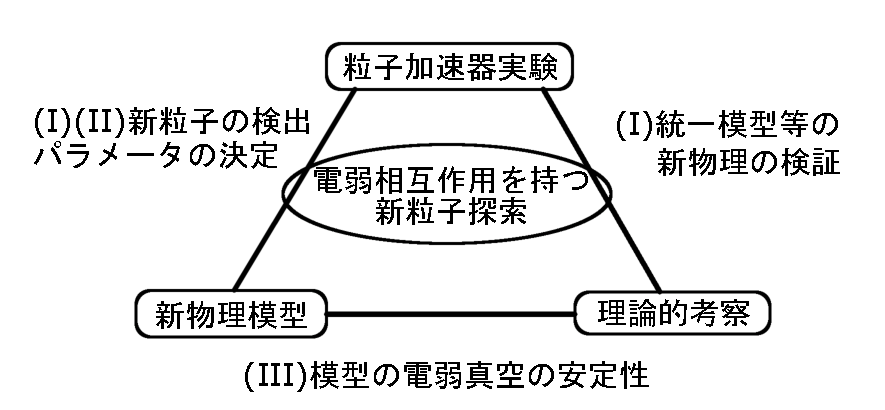
\includegraphics[width=\hsize]{figs/figure.pdf}
 \caption{本研究の全体像}
\end{wrapfigure}

粒子加速器を用いて電弱相互作用を持つ新粒子を探索し、その性質を調べること
を通じて、新物理模型への制限を与え、模型の妥当性を検証することが研究の目
的である。新粒子に対する感度を上げる工夫として、まず「I. 消失飛跡を用い
た新物理の性質の調査」に着目する。同時に「II. 標準模型の精密測定を用いた
新物理の探索」についても議論する。また「III. 電弱真空の安定性から導かれ
るより一般の素粒子模型への制限」の研究も行う。
%%
\vspace*{1mm}

\noindent{\fcolorbox{black}{my_gray}{具体的な研究目的と方法、内容}}

\vspace*{1mm}

\noindent{■ \emph{\ul{{\textbf{I.}} 消失飛跡を用いた新物理の性質の調査}}}

\vspace*{1mm}

\noindent{◆ \emph{\ul{研究目的、方法}}}

\vspace*{1mm}

$100\,\mathrm{TeV}$粒子加速器における消失飛跡の信号を用いることで、AMSB
模型に加え、その背後にある超対称性の破れのメカニズムや、統一模型などの物
理模型の正当性を検証することが目的である。現在までの研究で一部の新粒子の
質量の測定法を与えたが、それに加えて荷電Winoの寿命や、gluinoからBinoもし
くはWinoへの崩壊の分岐比に着目し、模型についてさらなる情報を引き出すこと
を目指す。

\vspace*{1mm}

\noindent{\emph{\ul{{\textbf{I-i.}} 長寿命粒子の寿命測定}}}

\vspace*{1mm}

\emph{【背景】}荷電Winoの寿命は質量の関数として詳細に計算されている。一
方、加速器実験における消失飛跡の信号は、一般には長寿命新粒子の存在を示す
のみであり、それをWinoと同一視するためには寿命の情報が必要となる。得ら
れた質量と寿命とを比較することで、AMSB模型の検証が可能となる。

\emph{【内容】}シミュレーションで生成された各荷電Winoに対し、ある寿命の
値に対応する確率分布から飛距離を計算し、実験のセットアップと比較すること
で、何層の検出器を通過したかを調べる。これを仮想的に実験データとみなし、
寿命の関数としてのイベント数の期待値と比較することで、寿命がどの程度の精
度で決定されるかを調べる。質量や寿命の測定誤差を考慮に入れて測定値を理論
曲線と比較し、どの程度まで模型の予言が検証できるか確かめる。

\vspace*{1mm}

\noindent{\emph{\ul{{\textbf{I-ii.}} {\textbf{gluino}} 崩壊分岐比の測定}}}

\vspace*{1mm}

\emph{【背景】}gluinoからBino、あるいはWinoへの崩壊の分岐比は、より重
いクォークの超対称パートナーの質量比によって決定される。そのため、実験
から分岐比を決めることで、実験の到達範囲を越えたエネルギースケールの物
理のヒントを得ることができる。この結果は、AMSB模型の背後にある物理模型
の検証に役立つ。

\emph{【内容】}実験でgluinoが生成された場合の最終的な信号は、Winoおよび
何本かの高エネルギージェットで特徴付けられる。gluinoの崩壊先の違いは高エ
ネルギージェットの本数の違いで観測が可能だが、その他にも過程の途中で多数
の低エネルギージェットがビーム軸の方向を中心に放出されていると予想される
ため、ジェットの運動量の大きさ、方向に対するカットを工夫し、最も正確に分
岐比を再構成できるカットの条件を調べる。

\vspace*{1mm}

\noindent{◆ \emph{\ul{展望}}}

\vspace*{1mm}

ここで決定された新物理の性質を元に理論的考察を行うことで、超対称性の破
れのメカニズムや、大統一理論などの統一模型との整合性を考察することが可
能となる。また、研究\textbf{I-ii.}のようなイベントの分類は、教師あり機
械学習が得意とする作業であり、これを用いた解析の改善も視野に入れている。
こういった機械学習の手法は電弱相互作用を持つ新粒子の研究のみならず、粒
子加速器実験の解析一般に応用が可能である。

\vspace*{1mm}

\noindent{■ \emph{\ul{{\textbf{II.}} 標準模型の精密測定を用いた新物理の探索}}}

\vspace*{1mm}

\noindent{◆ \emph{\ul{研究目的、方法}}}

\vspace*{1mm}

Higgsinoを始めとする電弱相互作用を持つ暗黒物質候補の検出が目的である。
現在までの研究で短寿命Higgsinoに有効な検出法を与えたが、暗黒物質の残存
量から示唆される質量を考えると、検出能力は未だ不十分である。そこでこの
手法の検出能力を引き上げるため、新たな標準模型過程を解析に加える。また、
新粒子の質量が大きい場合にも適用できる手法として、有効理論を用いた解析
を行い、様々な将来実験の検出能力の計算に適用する。

\vspace*{1mm}

\noindent{\emph{\ul{{\textbf{II-i.}} 電弱ゲージボソンの対生成過程を用いた新物理の探索}}}

\vspace*{1mm}

\emph{【背景】}電弱相互作用を持つ新粒子は量子補正を通じて電弱ゲージボ
ソンの対生成過程に影響を与えるため、これを用いて現在までの解析の検出能
力を引き上げることができる。一方、実験で実際に観測されるものは電弱ゲー
ジボソンが崩壊した後の粒子であるため、ゲージボソンの同定は容易でない。
この解析では非常に高エネルギーな終状態ゲージボソンが重要な役割を果たす
が、その崩壊先はおよそ同方向の運動量を持った複数の粒子であり、全体とし
て一つの太いジェットを構成する場合がある。このようなジェットはゲージボ
ソンの同定に用いることができる。

\emph{【内容】}電弱相互作用を持つ新粒子が過程に与える影響をループ計算
により求め、電弱ゲージボソン不変質量の関数としてどのような形を取るかを
調べる。ジェットを定義する太さのパラメータを変えながら、太いジェットの
解析でゲージボソンがどの程度同定できるかを調査する。対生成されたゲージ
ボソンの崩壊モード毎に、新粒子の存在にどの程度感度があるかを調べた上で、
レプトン対生成を用いた結果と全てを結合させ、最終的な検出能力を明らかに
する。

\vspace*{1mm}

\noindent{\emph{\ul{{\textbf{II-ii.}} 有効理論を用いた解析}}}

\vspace*{1mm}

\emph{【背景】}ILCやCLICに代表される、レプトン加速器の実験計画が数多く存
在する。これらは背景事象が比較的少なくクリーンな代わりに、衝突エネルギー
が低い傾向にある。このような場合の解析は、新物理の効果を積分して得られる
低エネルギー有効理論を用いて統一的に行うことができる。

\emph{【内容】}レプトン対生成やゲージボソン対生成を含めた、精密測定が
可能なプロセスに対し、寄与が大きい演算子を同定する。精密測定では多種の
系統誤差が寄与するので、それらの大きさにも注意を払いつつ、重要な演算子
の係数にどの程度の制限がつくかを調べる。最後にHiggsino等個々の模型に立
ち戻り、新粒子を積分して演算子の係数を決めるための関係式を導くことで、
有効理論への制限を模型の制限へと焼き直す。

\vspace*{1mm}

\noindent{◆ \emph{\ul{展望}}}

\vspace*{1mm}

本研究の手法は、標準模型と結合するあらゆる新物理の検出に応用可能である。
特に新粒子が短寿命、あるいは結合が弱いなどの理由で直接検出が難しい場合
に、この手法が効果を発揮する。また、現在稼働中のLHC等の実験がイベント
数の増加に伴い何らかのアノマリーを発見する可能性は大いにあり、有効理論
による解析結果があればそれらを各模型に関する予言へ言い換えることが可能
である。これらの結果は、本研究に適宜反映させる予定である。

\vspace*{1mm}

\noindent{■ \emph{\ul{{\textbf{III.}} 電弱真空の安定性から導かれるより一般の素粒子模型への制限}}}

\vspace*{1mm}

\noindent{◆ \emph{\ul{研究目的、方法}}}

\vspace*{1mm}

目的は超対称模型等、電弱対称性の破れを複数のスカラー場が担う模型に対し、
真空の安定性を保証する条件を導き、そこから模型への制限を与えることであ
る。特に研究\textbf{I.}の結果と組み合わせて、AMSB模型と思しき新物理が示
唆された場合にその性質に一貫性があるかを確認し、模型に対するさらなる制
限を得ることを考える。

\vspace*{1mm}

\noindent{◆ \emph{\ul{研究内容}}}

\vspace*{1mm}

まず超対称模型に着目する。崩壊率の計算に必要な関数が、運動方程式の非
自明な解として与えられる。経路積分を評価することにより、この関数を用い
て真空の崩壊率を与える表式を得る。この計算手法は、電弱対称性の破れの構
造がより複雑な別種の模型に対しても応用が可能であると考えられる。

%end  研究目的 ====================
}

%====================================
%form: pd_form_08.tex ; user: pd_08_plan.tex
%========== PD =========
%===== p. 08 年次計画 =============
\section{年次計画}
\subsection{年次計画}
\newcommand{\採用までの準備}{%
%begin  採用までの準備===================

\noindent{\fcolorbox{black}{white}{\emph{\textbf{I.} 消失飛跡を用いた新物理の性質の調査}}}

AMSB模型における荷電Winoの寿命と質量の間の関係式や、gluino崩壊分岐比の計
算を行う。またこれにより決まるパラメータと統一模型等のパラメータの間の関
係を、先行研究から理解する。これらの知識は、実験の結果を用いて模型を制限
する段階で必要となる。

\noindent{\fcolorbox{black}{white}{\emph{\textbf{II.} 標準模型の精密測定を用いた新物理の探索}}}

LHCの解析を参考にして伝統的な終状態ゲージボソンの同定法を理解し、シミュ
レーションの結果を用いて太いジェットを用いる手法と比較する。ここから、同
定の効率を最大化するために用いるべき手法や条件を求める。

%end  採用までの準備 ====================
}

\newcommand{\年次計画1年目}{%
%begin  年次計画1年目 (figureやtable使用可)===================

\vspace*{1mm}

\noindent{\fcolorbox{black}{white}{\emph{\textbf{I.} 消失飛跡を用いた新物理の性質の調査}}}

\vspace*{1mm}

研究内容の\textbf{I-i.}に対応する。シミュレーションで生成された各荷電
Winoに対し、飛距離をある確率分布に従う量として計算したものを、仮想的に実
験データとして解析を行う。得られたイベント数を理論値と比較することで寿命
の測定誤差を決定し、質量の測定誤差と考え合せることで、模型の予言がどの程
度まで検証されるかを調べる。

\vspace*{1mm}

\noindent{\fcolorbox{black}{white}{\emph{\textbf{II.} 標準模型の精密測定を用いた新物理の探索}}}

\vspace*{1mm}

研究内容の\textbf{II-i.}に対応する。電弱ゲージボソンの対生成過程に対して
電弱相互作用を持つ新粒子が与える影響を、ループダイアグラムを評価すること
で計算する。太いジェットを用いた解析で終状態ゲージボソンを同定し、得られ
たイベント数のセットを実験データとして解析を行う。フィットを用いる手法で
データから新粒子の影響を読み取り、統計処理を行うことで新粒子の検出能力を
計算する。

\vspace*{-5mm}

%end  年次計画1年目 (figureやtable使用可) ====================
}

\newcommand{\年次計画2年目}{%
%begin  年次計画2年目 (figureやtable使用可)===================

\vspace*{1mm}

\noindent{\fcolorbox{black}{white}{\emph{\textbf{I.} 消失飛跡を用いた新物理の性質の調査}}}

\vspace*{1mm}

研究内容の\textbf{I-ii.}に対応する。gluinoの崩壊モードを観測されたジェッ
トの本数を用いて区別するために、適切なジェットの運動量カットを調べる。最
適なカットがgluino質量を変化させた場合にどう振る舞うかを調べる。得られた
崩壊分岐比の決定誤差を模型内の重い新粒子の質量に対する条件に変換し、これ
を用いて模型に対する制限を得る。

\vspace*{1mm}

\noindent{\fcolorbox{black}{white}{\emph{\textbf{II.} 標準模型の精密測定を用いた新物理の探索}}}

\vspace*{1mm}

研究内容の\textbf{II-ii.}に対応する。レプトンやゲージボソンの対生成過程
に対して電弱相互作用を持つ新粒子が与える影響に着目し、影響の大きさの見積
もりに重要な演算子を同定する。重い新粒子を積分して、新粒子の質量や電荷と
演算子の係数との関係式を計算する。各演算子が実験のイベント数に与える影響
をシミュレーションから見積もり、演算子の係数に対する制限を得る。これを前
述の関係式と比較し、新粒子の性質がどの程度まで制限されるかを議論する。

\vspace*{1mm}

\noindent{\fcolorbox{black}{white}{\emph{\textbf{III.} 電弱真空の安定性から導かれるより一般の素粒子模型への制限}}}

\vspace*{1mm}

研究内容の\textbf{III.}に対応する。最小超対称模型に着目し、運動方程式の
非自明な解を計算する。この解の周辺の量子ゆらぎを経路積分を用いて足し上げ
ることで、この模型に対する真空の崩壊率の表式を得る。研究\textbf{I.}で得
られた模型パラメータの決定能力と組み合わせることで、模型の一貫性から模型
に与えられる制限を議論する。

\vspace*{-5mm}

%end  年次計画2年目 (figureやtable使用可) ====================
}

\newcommand{\年次計画3年目}{%
%begin  年次計画3年目 (figureやtable使用可)===================

\vspace*{1mm}

\noindent{\fcolorbox{black}{white}{\emph{\textbf{I.} 消失飛跡を用いた新物理の性質の調査}}}

\vspace*{1mm}

研究内容の\emph{\textbf{I-}将来の展望}に対応する。教師有り機械学習を用い
たイベントの分類のためのコードを用いて、gluinoの崩壊モードを同定する。得
られた結果を精査し、崩壊モードの同定に無関係な低エネルギージェットがどう
処理されているかを読みとる。前年度までの研究成果と比較することで、どのよ
うな解析が結果の改善に役立つかを議論する。

\vspace*{1mm}

\noindent{\fcolorbox{black}{white}{\emph{\textbf{III.} 電弱真空の安定性から導かれるより一般の素粒子模型への制限}}}

\vspace*{1mm}

引き続き研究内容の\textbf{III.}に対応する。前年度までの計算を応用して、
最小超対称模型に限らず、二つ以上のスカラー場が複雑な電弱対称性の破れを引
き起こす模型に対し、電弱真空の崩壊率の計算を行う。

\noindent{
◆ \emph{\ul{研究成果は逐次国内外の研究会で発表する。}}~~
◆ \emph{\ul{本研究中に発表される実験の結果は適宜内容に反映させる。}}
}

%end  年次計画3年目 (figureやtable使用可) ====================
}

%    }
%form: pd_form_09.tex ; user: pd_09_rights.tex
%========== PD =========
%===== p. 09 人権の保護及び法令等の遵守への対応 =============
\subsection{人権の保護及び法令等の遵守への対応}
\newcommand{\受け入れ研究室の選定理由}{%
%begin  受け入れ研究室の選定理由===================

■ \emph{\ul{知るきっかけ、打ち合わせ状況}}

\vspace*{1mm}

受入研究者である遠藤氏は超対称模型や暗黒物質、有効理論を用いた精密計算な
ど、幅広い分野に渡って精力的に研究を行なっている研究者である。同時に遠藤
氏は、近年における電弱真空崩壊率の精密計算の第一人者でもある。申請者が研
究を行う際、これらの研究を参考としたことが、知るきっかけである。また申請
者はKEKで自身の研究に関するセミナーを行い、その際遠藤氏と申請者の研究内
容について議論した。加えて、その他研究会等においても遠藤氏との議論の経験
があるため、共同研究は支障なく行えると考えられる。

\vspace*{1mm}

■ \emph{\ul{メリット、新たな発展・展開}}

\vspace*{1mm}

上記の通り遠藤氏は超対称模型や暗黒物質、有効理論による計算、電弱真空崩壊
率の計算などに関して幅広い知識を持っている。そのため、研究課題I、IIで新
粒子探索から得られる模型への制限を考える際、議論を通じて知識を共有し、研
究をより洗練することが可能であると考えられる。また、研究課題IIIのような
種々の模型における真空崩壊率の精密計算を行う際、その計算手法を確立した遠
藤氏と議論しつつ研究を進められることは、申請者にとってのメリットである。
加えて受入研究機関のKEKには、宇宙論や量子場のダイナミクス等、様々な分野
に精通する優れた研究者が複数在籍している。彼らとの議論を通じ、新たな視点
を手に入れることで、上記の計画以上の新たな発展も期待できる。

%end  受け入れ研究室の選定理由 ====================
}

\newcommand{\人権の保護及び法令等の遵守への対応}{%
%begin  人権の保護及び法令等の遵守への対応 ===================

該当しない。

%end  人権の保護及び法令等の遵守への対応 ====================
}

%form: pd_form_10-11.tex ; user: pd_10-11_publications.tex
%========== PD =========
%===== p. 10-11 研究業績 =============
\section{研究業績}
%watermark: w14_pub_pd
% 2008-03-08 Taku
% 2009-03-04 K.S.
% 2010-05-06 Taku
% 2017-03-02 Taku: Added \KLCheckPageLimit and \KLAdvancePages.
\subsection{学術雑誌(紀要・論文集等も含む)に発表した論文及び著書}
\newcommand{\学術雑誌等に発表した論文または著書}{%
%begin  学術雑誌等に発表した論文または著書===================
	
	\begin{enumerate}
	 \item[](査読有り)%===========================
	 \item \ul{S.~Chigusa} and T.~Moroi,
	       ``Bottom-tau unification in a supersymmetric model with anomaly-mediation,''
	       Phys.\ Rev.\ D {\bf 94} (2016) no.3,  035016
	 \item \ul{S.~Chigusa} and T.~Moroi,
	       ``Bottom-Tau Unification in Supersymmetric SU(5) Models with Extra Matters,''
	       PTEP {\bf 2017} (2017) no.6,  063B05
	 \item \ul{S.~Chigusa}, T.~Moroi and Y.~Shoji,
	       ``State-of-the-Art Calculation of the Decay Rate of Electroweak Vacuum in the Standard Model,''
	       Phys.\ Rev.\ Lett.\  {\bf 119} (2017) no.21,  211801
	 \item \ul{S.~Chigusa}, T.~Moroi and Y.~Shoji,
	       ``Decay Rate of Electroweak Vacuum in the Standard Model and Beyond,''
	       Phys.\ Rev.\ D {\bf 97} (2018) no.11,  116012
	 \item \ul{S.~Chigusa} and K.~Nakayama,
	       ``Anomalous Discrete Flavor Symmetry and Domain Wall Problem,''
	       Phys.\ Lett.\ B {\bf 788} (2019) 249
	 \item \ul{S.~Chigusa}, S.~Kasuya and K.~Nakayama,
	       ``Flavon Stabilization in Models with Discrete Flavor Symmetry,''
	       Phys.\ Lett.\ B {\bf 788} (2019) 494
	 \item \ul{S.~Chigusa}, Y.~Ema and T.~Moroi,
	       ``Probing electroweakly interacting massive particles with Drell–Yan process at 100 TeV hadron colliders,''
	       Phys.\ Lett.\ B {\bf 789} (2019) 106
	 \item S. Asai, \ul{S. Chigusa}, T. Kaji, T. Moroi, M. Saito,
	       R. Sawada, J. Tanaka, K. Terashi and K. Uno,
	       ``Studying gaugino masses in supersymmetric model at future 100 TeV $pp$ collider,''
	       \rem{Biblio??}

		       

		\item[](査読なし)%=============================

		       なし
		       
	\end{enumerate}
%end  学術雑誌等に発表した論文または著書 ====================
}

\subsection{学術雑誌等又は商業誌における解説・総説}
\newcommand{\学術雑誌等または商業誌における解説や総説}{%
%begin  学術雑誌等または商業誌における解説や総説===================

なし

%end  学術雑誌等または商業誌における解説や総説===================
}

\subsection{国際会議における発表}
\newcommand{\国際会議における発表}{%
%begin  国際会議における発表===================

(口頭、査読有り)
	\begin{enumerate}
	 \item \ul{S. Chigusa}${}^\circ$ and T. Moroi, 
	       ``Bottom-Tau unification in Supersymmetric Model with Anomaly-Mediation'',
	       SUSY 2016,
	       The University of Melbourne (Australia),
	       2016年7月
	 \item \ul{S. Chigusa}${}^\circ$ and T. Moroi,
	       ``Bottom-Tau Unification in Supersymmetric Models'',
	       New Physics Forum,
	       IPMU,
	       2017年2月
	 \item \ul{S. Chigusa}${}^\circ$, T. Moroi and Y. Shoji,
	       ``Decay Rate of the Electroweak Vacuum in the Standard Model and Beyond'',
	       Planck 2018,
	       University of Bonn (Germany),
	       2018年5月
	 \item \ul{S. Chigusa}${}^\circ$ and K. Nakayama,
	       ``Flavon Stabilization in Models with Discrete Flavor Symmetry'',
	       KEK-PH 2018 winter
	       KEK,
	       2018年12月	      
	\end{enumerate}
(ポスター、査読有り)
        \begin{enumerate}
	 \setcounter{enumi}{4}
	 \item \ul{S. Chigusa}${}^\circ$ and T. Moroi,
	       ``Bottom Tau Unification in Supersymmetric Models'',
	       Les Houches Summer School 2017,
	       Les Houches School of Physics (France),
	       2017年7月
	 \item \ul{S. Chigusa}${}^\circ$, T. Moroi and Y. Shoji,
	       ``Decay Rate of the Electroweak Vacuum in the Standard Model and Beyond'',
	       Cargese 2018 International Summer School,
	       Scientific Institute of Cargese (France),
	       2018年7月
	 \item \ul{S. Chigusa}${}^\circ$, Y. Ema and T. Moroi
	       ``Probing Electroweakly Interacting Massive Particles with Precision Measurements at 100 TeV Hadron Colliders'',
	       Higgs as a Probe of New Physics 2019,
	       Osaka University,
	       2019年2月
	\end{enumerate}
%end  国際会議における発表 ====================
}

\subsection{国内学会・シンポジウムにおける発表}
\newcommand{\国内学会やシンポジウムにおける発表}{%
%begin  国内学会やシンポジウムにおける発表===================
(口頭、査読有り)
	\begin{enumerate}
	 \item \ul{S. Chigusa}${}^\circ$ and T. Moroi,
	       ``Bottom-Tau unification in Supersymmetric Model with Anomaly-Mediation'',
	       日本物理学会秋季大会,
	       宮崎大学,
	       2016年9月
	 \item \ul{S. Chigusa}${}^\circ$, T. Moroi and Y. Shoji,
	       ``Zero Mode Problem in the Calculation of Decay Rate of the SM Electroweak vacuum'',
	       日本物理学会秋季大会,
	       信州大学,
	       2018年9月
	\end{enumerate}
(ポスター、査読有り)
         \begin{enumerate}
	  \setcounter{enumi}{2}
	  \item \ul{S. Chigusa}${}^\circ$ and T. Moroi,
		``Bottom Tau Unification in Supersymmetric Models'',
		素粒子物理学の進展 2017,
		京都大学,
		2017年8月
	  \item \ul{S. Chigusa}${}^\circ$, Y. Ema and T. Moroi
		``Indirect Search of WIMP Dark Matter at Future 100 TeV Collider'',
		素粒子物理学の進展 2018,
		京都大学,
		2018年8月
	 \end{enumerate}
%end  国内学会やシンポジウムにおける発表 ====================
}

\subsection{特許等}
\newcommand{\特許等}{%
% %begin  特許等===================

なし

% %end  特許等 ====================
}

\subsection{その他の業績}
\newcommand{\その他の業績}{%
%begin  その他の業績===================

(受賞歴)
\begin{enumerate}
 \item 国際会議 ``Higgs as a Probe of New Physics
       2019'' において、the Best Poster Award 受賞(発
       表 4-(3)-7 に基づく)
\end{enumerate}

(arXiv 投稿済、査読中)
\begin{enumerate}
 \setcounter{enumi}{1}
 \item T. Abe, \ul{S. Chigusa}, Y. Ema and T. Moroi
       ``~~~~''
       \rem{Preprint??}
\end{enumerate}

(対外講演)
\begin{enumerate}
 \setcounter{enumi}{2}
 \item 名古屋大学(2018/10/16)、北海道大学(2019/1/11)、KEK
       (2019/4/9)で自身の研究内容に関するセミナーを行った。また、フ
       ロリダ州立大学(2019/5/10)、フロリダ大学(2019/5/16)でもセミ
       ナーを行う予定である。
\end{enumerate}

(その他)
\begin{enumerate}
 \setcounter{enumi}{3}
 \item 学術振興会特別研究員 DC1 に採択:2017年4月--2020年3月
 \item 東京大学数物フロンティア・リーディング大学院(FMSP)のコース生
       に採択:2015年10月--2020年3月
\end{enumerate}
%end  その他の業績 ====================
}

%===========================================================
% hook9 : right before \end{document} ============

%endUserFiles
% hook7 : right before including forms ============
 % for future maintenance

% pd_forms
%=======================================
\ifthenelse{\boolean{BudgetSummary}\OR\boolean{klTypesetPage0}}{
	%============================================================
%  Warning cover page
%============================================================

\begin{picture}(0,0)(\KLOddPictureX,\KLPictureY)
	\KLParbox{100}{700}{550}{600}{t}{
		\LARGE
		提出前に次の行を以下のようにコメントアウトし、\\
		コンパイルし直してください。\\
		\hspace{2cm}\%\textbackslash setboolean\{BudgetSummary\}\{true\}\\
		\hspace{2cm}\%\textbackslash KLTypesetPage\{..\}\\
		\hspace{2cm}\%\textbackslash KLTypesetPagesInRange\{..\}\{..\}\\
	}
	\西暦
	\KLParbox{100}{550}{500}{500}{t}{
		\begin{center}
			\LARGE 予算と研究組織のまとめ \\
			\Large \today
		\end{center}
	}

	\KLTextBox{100}{500}{550}{300}{}{
		\Large
		研究種目: \研究種目\研究種別\研究種目後半\\
		研究期間: \研究開始年度(H\研究開始元号年度) 〜 H\研究期間の最終元号年度\\
		研究課題名:「\研究課題名」\\
		研究代表者:\研究代表者氏名\\
		研究機関名:\研究機関名\\
	}
\end{picture}
\clearpage


}{}

\KLInputIfPageInRangeIsSelected{1}{2}{forms/pd_form_03-04}
\KLInputIfPageInRangeIsSelected{3}{5}{forms/pd_form_05-07}
\KLInputIfSelected{6}{forms/pd_form_08}
\KLInputIfSelected{7}{forms/pd_form_09}
\KLInputIfPageInRangeIsSelected{8}{9}{forms/pd_form_10-11}

%========================================


%endFormatFile

% hook9 : right before \end{document} ============
 % for future maintenance
\end{document}
